% !TEX root=/home/tavant/these/manuscript/src/manuscript.tex

\section{Axial-azimuthal \acs{2D} \acs{PIC} simulation}
  \label{sec-axial-azimuthal}
  
  The radial and azimuthal simulation allows us to study the plasma-wall interaction coupled with the self-consistent azimuthal instability.
  As previously mentioned, however, axial gradients are missing (magnetic field, densities, temperatures, etc.) as well as the axial convection of the wave and the particles.
  In order to study those phenomena, the axial and azimuthal simulation domain is used \citep{adam2004,coche2014,lafleur2018,boeuf2018}.
  \Cref{fig-2Dz} shows a schematic representation of this simulation domain.
  In this configuration, the anode side is set $U_d$ the discharge voltage, and the cathode side is grounded.
  
  
  
  \begin{figure}[hbt]
    \centering
    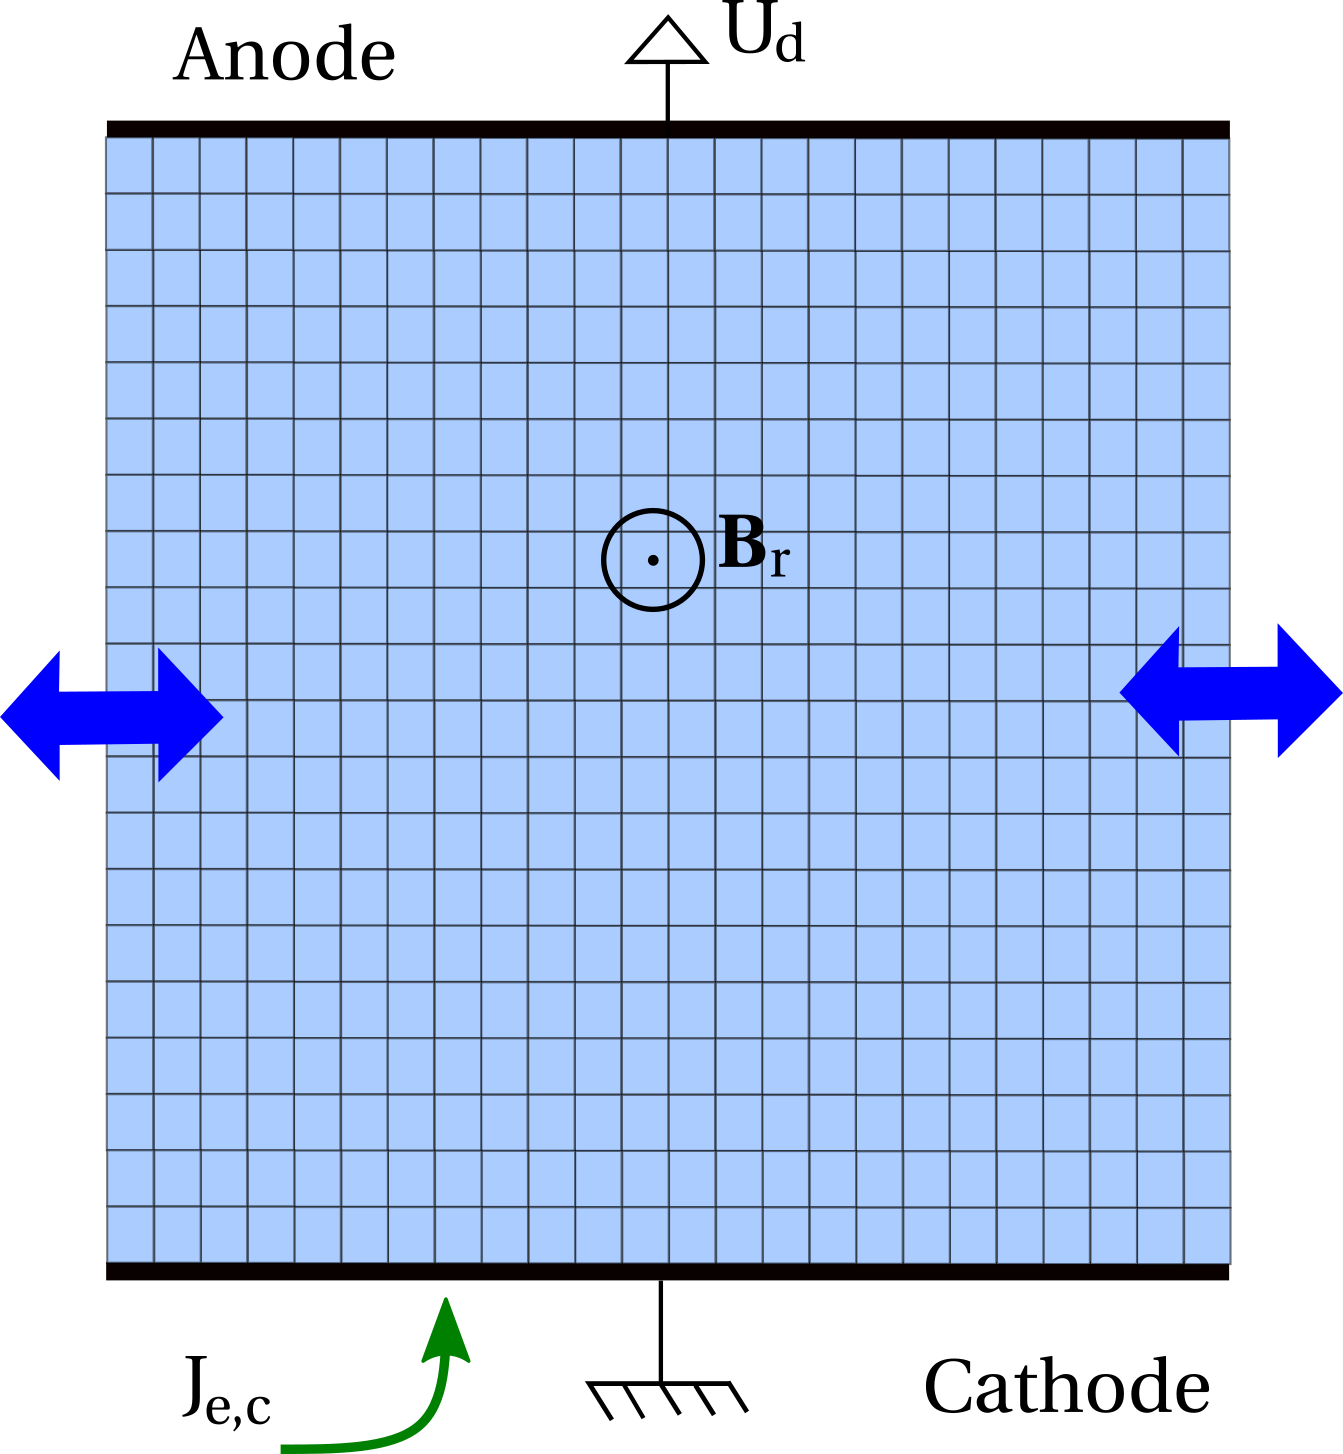
\includegraphics[width=0.5\textwidth]{2D_Ztheta.png}
    \caption{Schematic representation of the axial and azimuthal simulation domain. $U_d$ is the voltage imposed at the anode (of the order of $300\,\volt$) and $J_{e,c}$ correspond to the electrons emitted by the grounded cathode, used to initiate and maintain the plasma discharge. Periodic boundary conditions are used in the azimuthal direction. A radial magnetic field $B_r$ is imposed, which amplitude depends on the axial position. }
    \label{fig-2Dz}
  \end{figure}
  A radial magnetic field is imposed, that amplitude follows an axial profile such as in \cref{fig-bshape}.
  The axial electric field is self-consistently computed by solving the Poisson equation.
  In this configuration, one need to injected a flux of electron $J_{e,c}$ corresponding to the contribution of the cathode to sustain the plasma.
  While this configuration models the physics of the axial direction, it does not model the plasma-wall interaction.
  In \cref{ch-6}, we propose an algorithm to model the effects of the walls on the particle and power balance.
  The principal idea is to model the absorption  of the particles by the wall in a fashion similar to the axial convection of particle used in the radial-azimuthal simulation (described in \cref{sec-reinjectionnoise}).
  
  More informations of the axial-azimuthal simulation domain and the radial losses algorithm are given in \Cref{ch-6}.
  
  